\documentclass[aspectratio=169]{beamer}

% Bibliography (if needed)
\usepackage[backend=biber,style=apa]{biblatex}
\addbibresource{refs.bib}

% Math and Graphics
\usepackage{amsmath}
\usepackage{graphicx}
\usepackage{tikz}
\usepackage{booktabs}
\usetheme{metropolis}
\usepackage{caption}

% Title Info
\title{Nepali Sentiment Analysis of Post-COVID Data}
\subtitle{Using XLMRoberta for Text Classification}
\author{Amulya Bhandari \and Sailesh Dahal \and Sarayu Gautam \and Tohfa Niraula}
\institute{Department of Computer Engineering\\Kathmandu University}
\date{\today}

\begin{document}

% Title Slide
\maketitle

% Outline
\begin{frame}{Outline}
  \tableofcontents
\end{frame}

% Introduction
\section{Introduction}
\begin{frame}{What is Sentiment Analysis?}
  \begin{itemize}
    \item Sentiment analysis classifies text based on emotion or opinion \parencite{article}.
    \item Categories:
          \begin{itemize}
            \item Positive — praise, approval
            \item Neutral — factual
            \item Negative — criticism, disapproval
          \end{itemize}
    \item Applications:
          \begin{itemize}
            \item Social media monitoring
            \item Product reviews
            \item Survey analysis
          \end{itemize}
  \end{itemize}
\end{frame}

% Problem Statement
\section{Problem Statement}
\begin{frame}{What Are We Solving?}
  \begin{itemize}
    \item Goal: Classify Nepali-language text into sentiment categories.
    \item Motivation:
          \begin{itemize}
            \item Nepali is underrepresented in NLP.
            \item Enhance Accessibility for Nepali Language.
          \end{itemize}
    \item Objectives:
          \begin{enumerate}
            \item Clean and preprocess post-COVID Nepali data.
            \item Train a multilingual BERT model.
            \item Evaluate performance using real-world test data.
          \end{enumerate}
  \end{itemize}
\end{frame}

% Dataset Description
\section{Dataset Description}
\begin{frame}{About the Dataset}
  \begin{columns}[T]
    % Left column for text
    \begin{column}{0.5\textwidth}
      \begin{itemize}
        \item Source: Nepali COVID/post-COVID text samples \parencite{aayam_ojha_2023,ajhesh72022nepali,shushant2021nepalisentiment,mahesh2022nepali}.
        \item Total Samples:
              \begin{itemize}
                \item Training: 33,602 samples
                \item Testing: 8,401 samples
              \end{itemize}
        \item Labels: 0 = Negative, 1 = Positive, 2 = Neutral
        \item Common issues:
              \begin{itemize}
                \item Invalid labels ('o', '-', etc.)
                \item Missing values and noisy characters
              \end{itemize}
      \end{itemize}
    \end{column}

    % Right column for figure
    \begin{column}{0.45\textwidth}
    \centering
      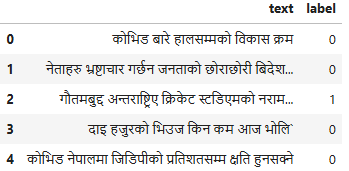
\includegraphics[width=\textwidth]{DataSample.png}
      \captionof{figure}{Data Sample}
    \end{column}
  \end{columns}
\end{frame}

% Preprocessing
\section{Data Preprocessing}
\begin{frame}{Data Cleaning Steps}
  \begin{columns}[T]
    % Left column for text
    \begin{column}{0.5\textwidth}
      Steps we took:
      \begin{enumerate}
        \item Removed missing and malformed data.
        \item Filtered invalid labels.
        \item Tokenized using XLM-Roberta tokenizer.
        \item Truncated inputs to max length of 256 tokens.
      \end{enumerate}
      Result: Clean, structured datasets ready for training/testing.
    \end{column}

    % Right column for figure
    \begin{column}{0.25\textwidth}
    \centering
      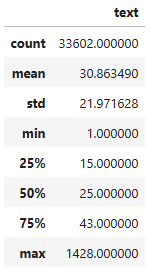
\includegraphics[width=\textwidth]{TruncateReason.png}
      \captionof{figure}{ Data Length}
    \end{column}
  \end{columns}
\end{frame}

% Tokenization and Encoding
\section{Tokenization and Encoding}
\begin{frame}{Tokenizing with XLM-Roberta}
  \begin{itemize}
    \item XLM-Roberta tokenizer is multilingual and supports Nepali language \parencite{conneau-etal-2020-unsupervised}.
    \item Key features of \texttt{tokenizer.batch\_encode\_plus}:
          \begin{itemize}
            \item Automatically handles padding and truncation for consistent input length.
            \item Generates:
                  \begin{itemize}
                    \item \texttt{input\_ids}: Numerical representation of tokens.
                    \item \texttt{attention\_mask}: Identifies non-padded tokens for focus.
                  \end{itemize}
          \end{itemize}
    \item Attention masks ensure the model processes only relevant tokens. It tells the model which sentence is real and which is padding.
  \end{itemize}
\end{frame}
\begin{frame}{Understanding Tokenization and Encoding}
  \begin{itemize}
    \item Tokenizing is like chopping a sentence into Lego blocks that the model knows.
    \item Encoding is turning those blocks into numbers so the model can do math with them.
    \item Why It Matters:
          \begin{itemize}
            \item The model sees only numbers.
            \item Tokenization keeps input size fixed (e.g., max\_length=256). Long texts are trimmed, short ones are padded.
          \end{itemize}
  \end{itemize}
\end{frame}

\begin{frame}{Tokenization Example}
  \centering
  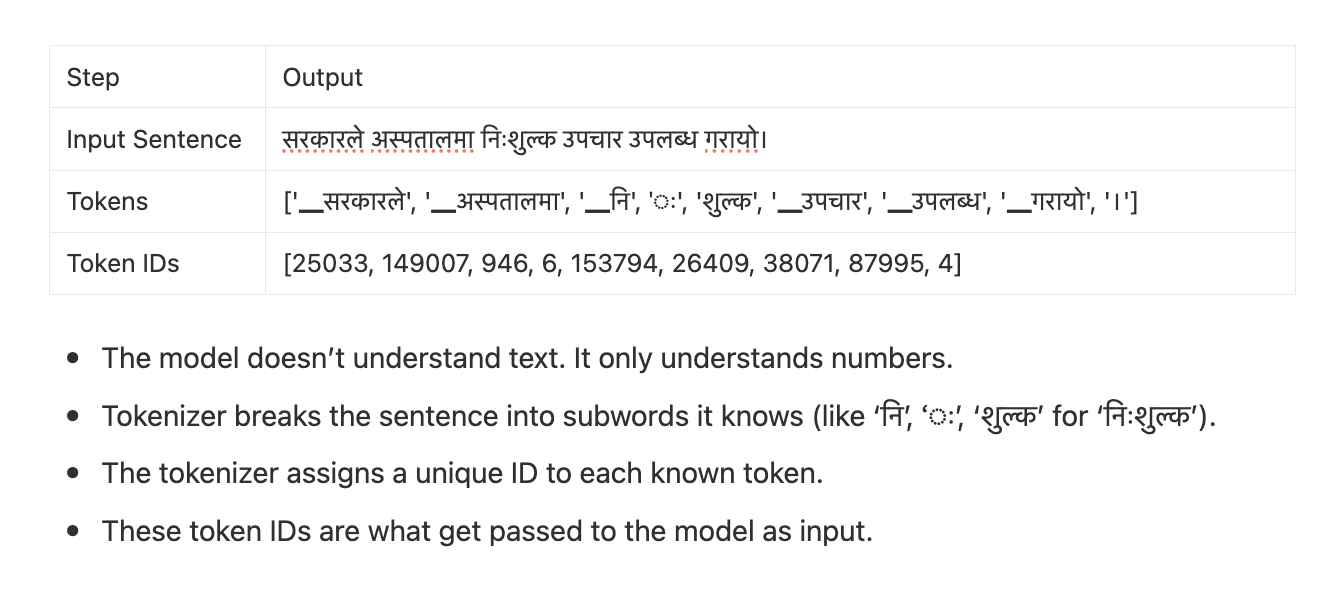
\includegraphics[width=1\linewidth]{example.png}
    \captionof{figure}{ Tokenization Example}
\end{frame}

% Model Architecture
\section{Model Architecture}
\begin{frame}{XLM-Roberta Model Details}
  Transformers process all words at the same time (not one-by-one like RNN) \parencite{vaswani2023attentionneed}.

  Structure:
  \begin{itemize}
    \item XLM-R supports multiple languages, including Nepali, out of the box \parencite{conneau-etal-2020-unsupervised}.
    \item Fine-tuning was performed to adapt the model's top layers specifically for sentiment classification \parencite{devlin-etal-2019-bert,liu2019roberta}.
    \item Produces probabilities for three sentiment classes: Negative, Positive, and Neutral.
  \end{itemize}

  Trained on: PyTorch with mixed precision (autocast enabled) \parencite{paszke2019pytorchimperativestylehighperformance,priya2020mixed}
\end{frame}

\begin{frame}{Model Usage Example}
  \centering
  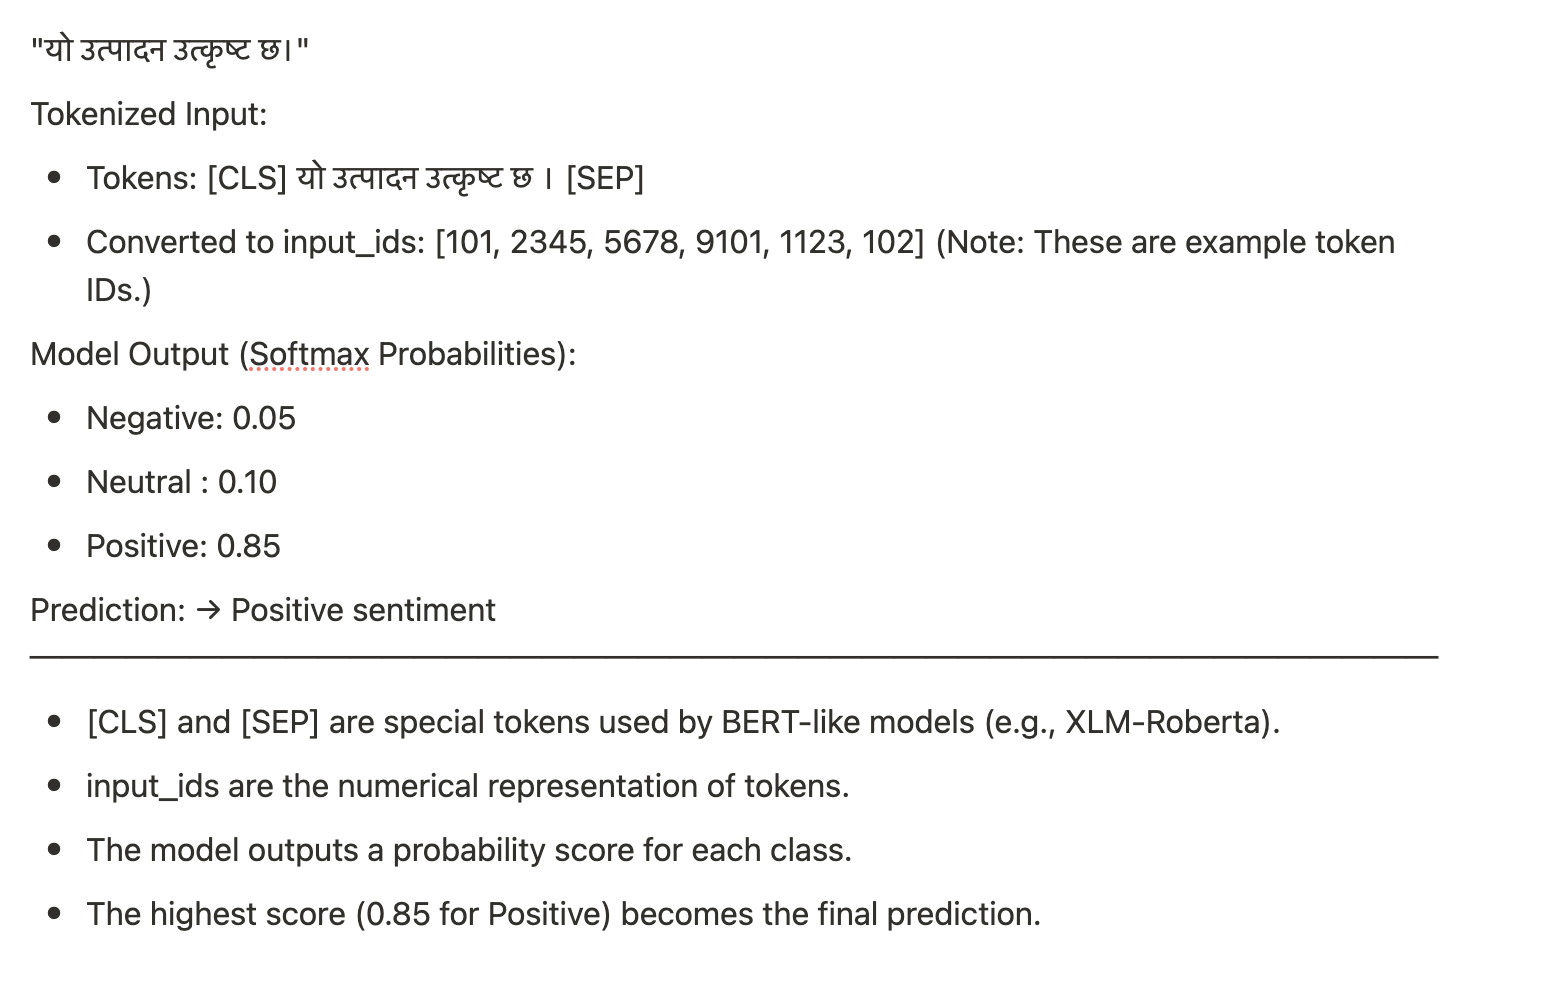
\includegraphics[width=0.65\linewidth]{example2.png}
    \captionof{figure}{Model Usage Example}
\end{frame}


% Training Pipeline
\section{Training Pipeline}
\begin{frame}{Main Workflow Steps}
  \centering
  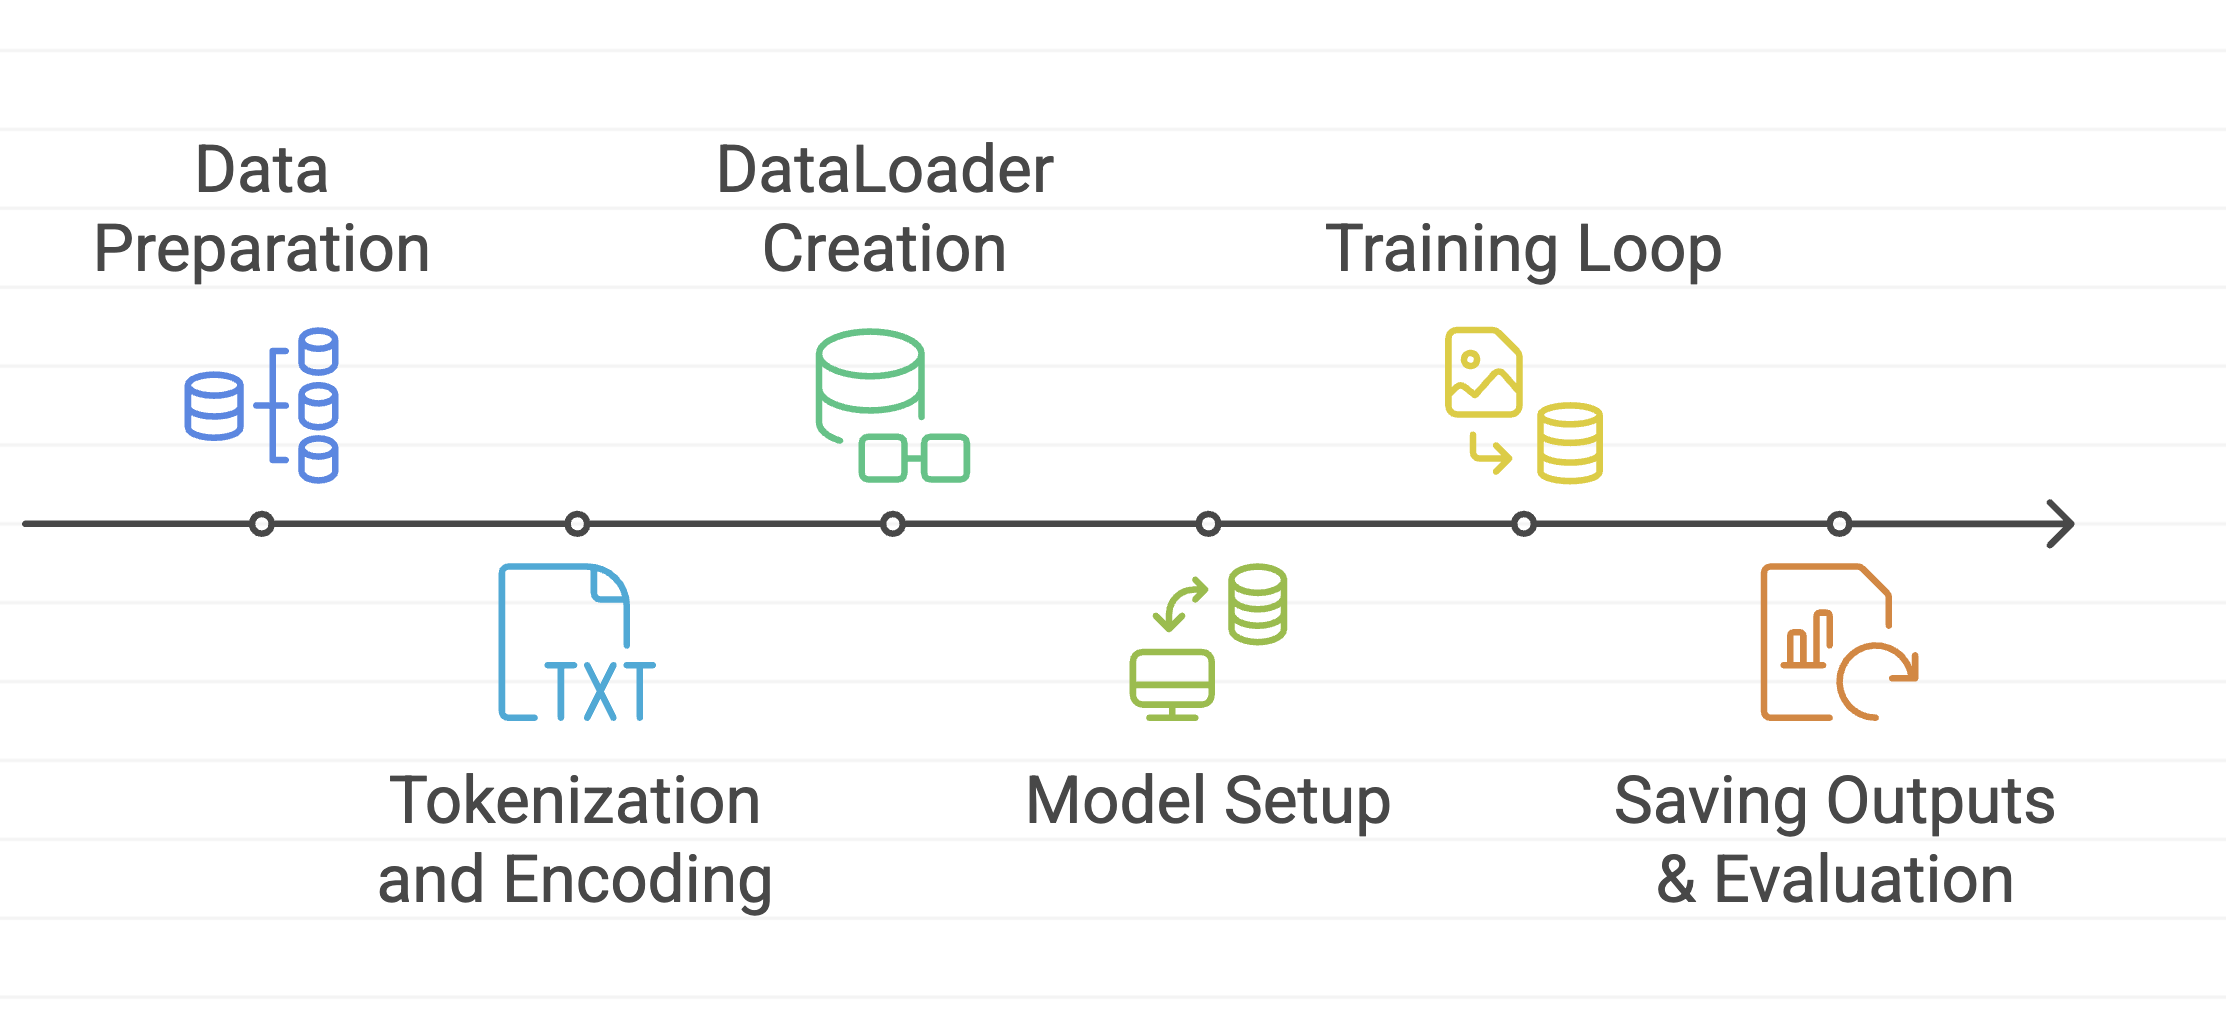
\includegraphics[width=0.95\linewidth]{workflow.png}
    \captionof{figure}{ Workflow Steps}

\vspace{-0.5em}
\footnotesize{Implementation using PyTorch \parencite{paszke2019pytorchimperativestylehighperformance} and Transformers library \parencite{wolf-etal-2020-transformers}}
\end{frame}

\begin{frame}{Training Loop}
  \centering
  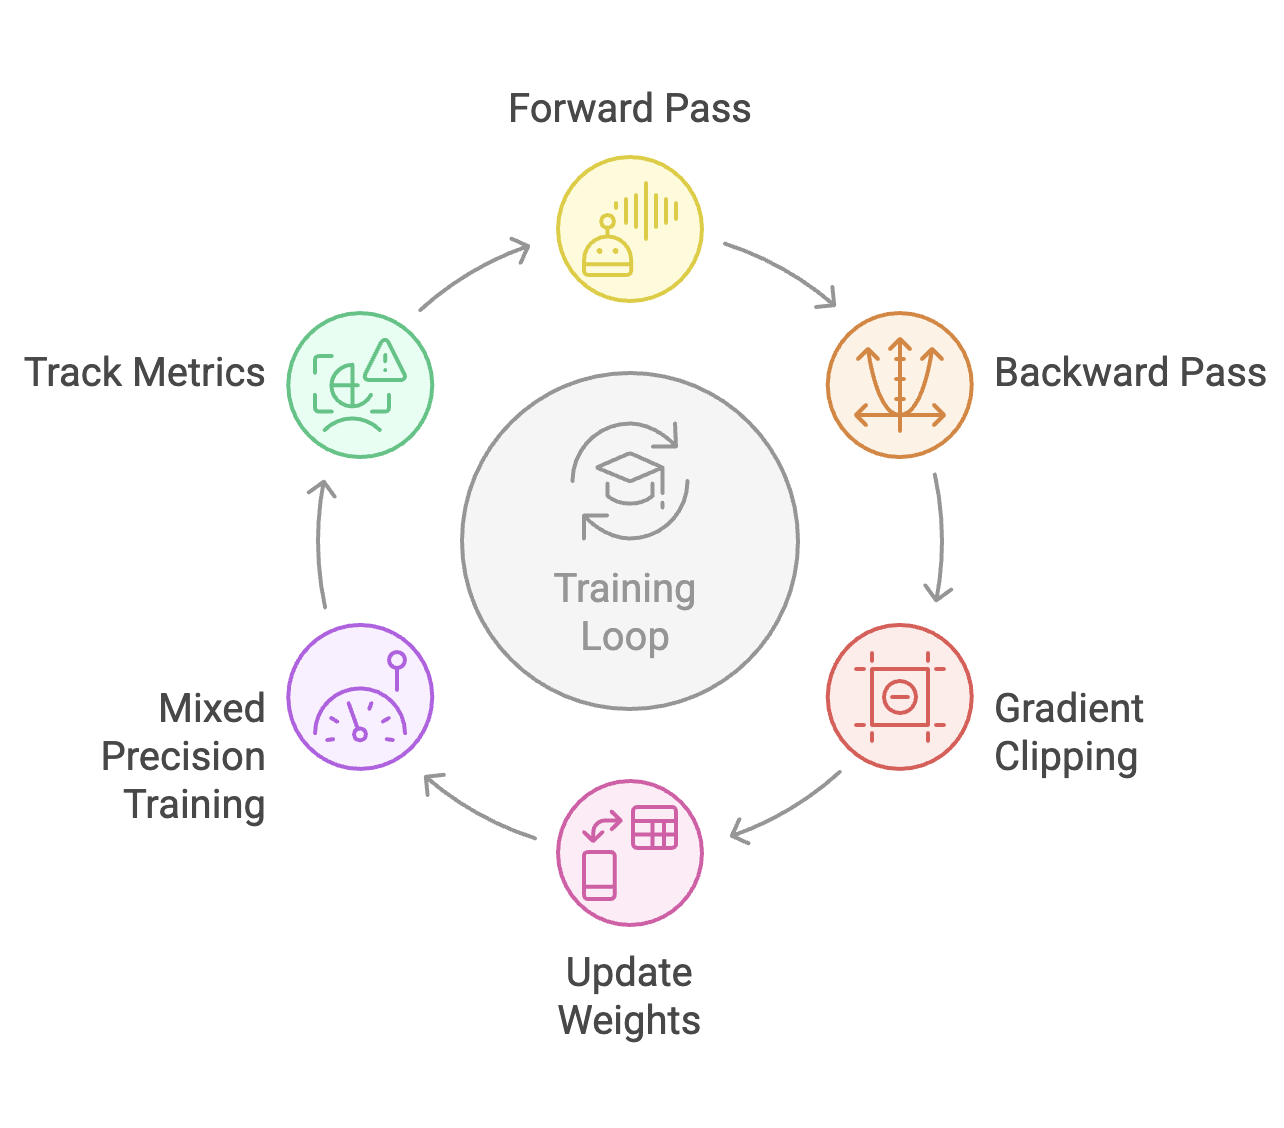
\includegraphics[width=0.55\linewidth]{trainLoop.png}
    \captionof{figure}{ Training Loop}

\footnotesize{Optimizer: AdamW \parencite{loshchilov2019decoupledweightdecayregularization}}
\end{frame}

\begin{frame}{Deployment and Evaluation}
  \centering
  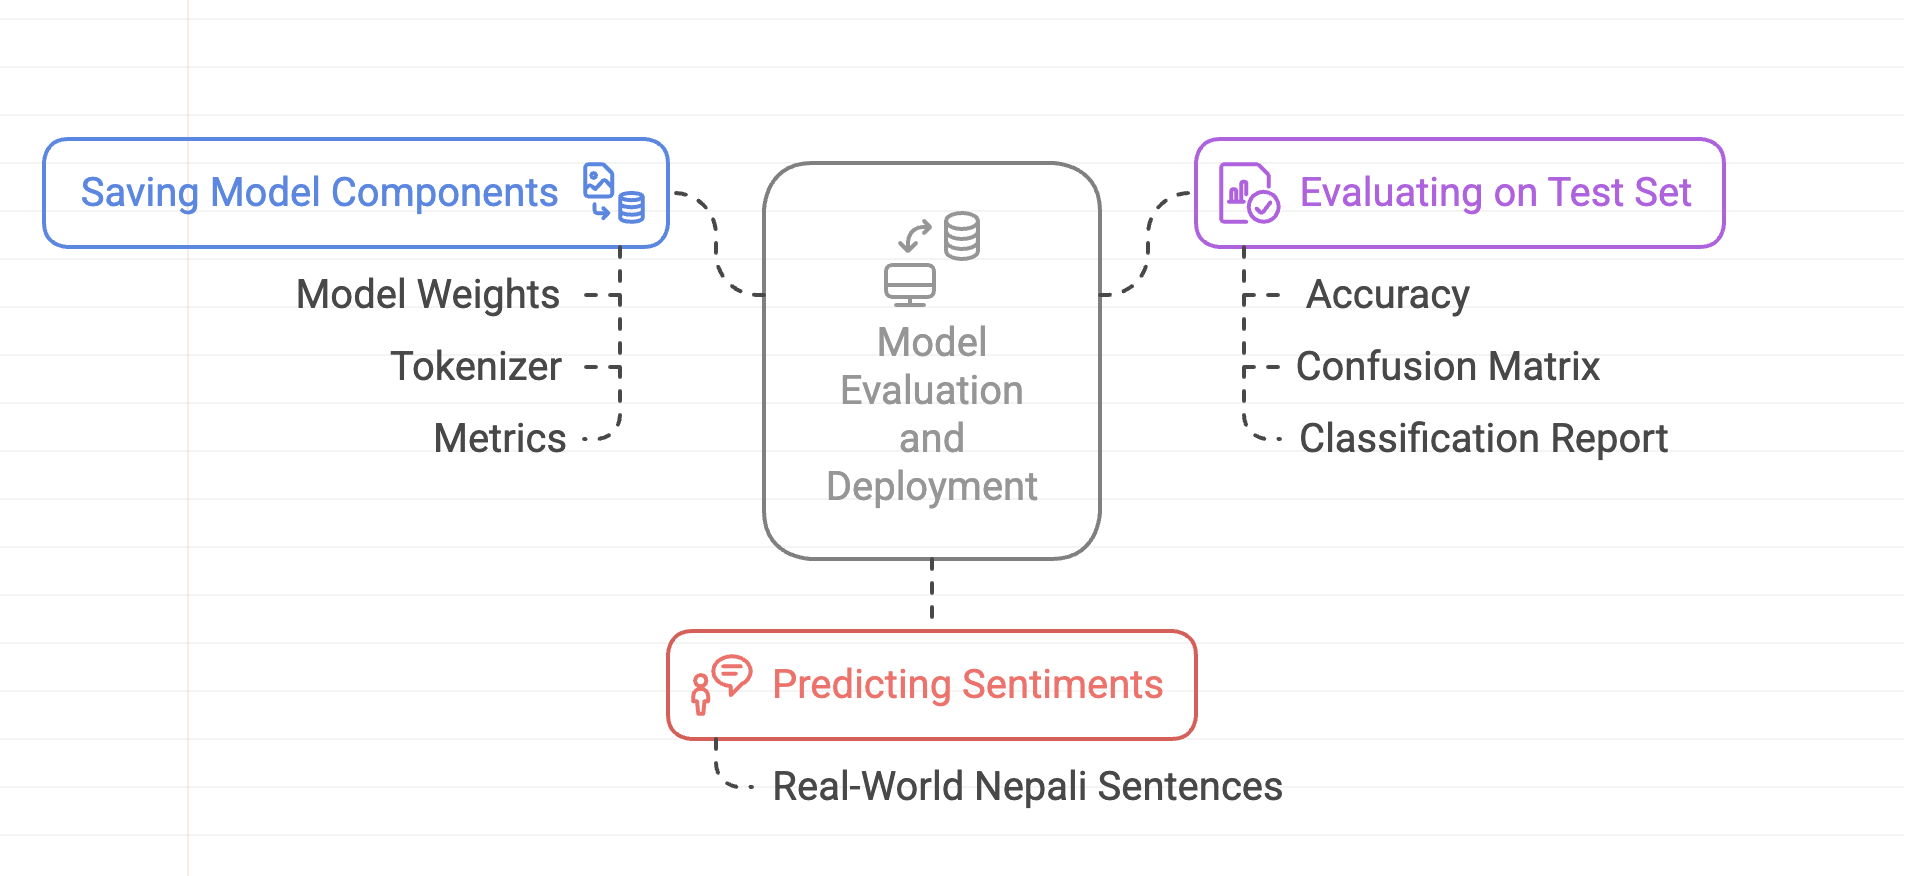
\includegraphics[width=0.95\linewidth]{deployment.png}
    \captionof{figure}{ Deployment}
\end{frame}

% Results Plot
\section{Results}
\begin{frame}{Loss and Accuracy Over Epochs}
  \centering
  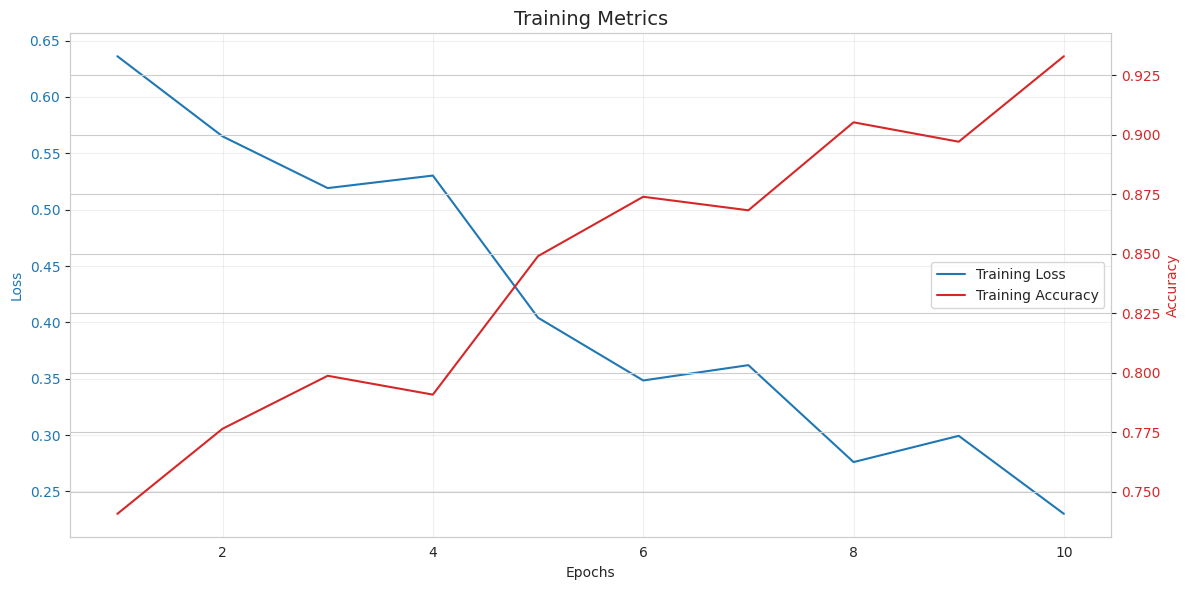
\includegraphics[width=0.75\linewidth]{training_metrics.png}
    \captionof{figure}{ Loss and Accuracy}
\end{frame}

% Classification Report
\begin{frame}{Test Set Evaluation Metrics}
  \vspace{-0.5em}
  {\small
    \begin{tabular}{lccc}
      Label            & Precision & Recall & F1-score     \\
      \hline
      Negative (0)     & 0.80      & 0.74   & 0.77         \\
      Positive (1)     & 0.78      & 0.83   & 0.80         \\
      Neutral (2)      & 0.52      & 0.52   & 0.52         \\
      \\[-0.8em]
      Overall Accuracy &           &        & {\bf 74.0\%} \\
    \end{tabular}}

  \vspace{1em}

  Key Insights:
  \begin{itemize}
    \item High precision/recall for Positive/Negative.
    \item Neutral class more ambiguous → lower performance.
  \end{itemize}
\end{frame}

% Confusion Matrix Image (Optional)
\begin{frame}{Model Performance on Test Set}
  \begin{columns}
    \begin{column}{0.5\textwidth}
      \centering
      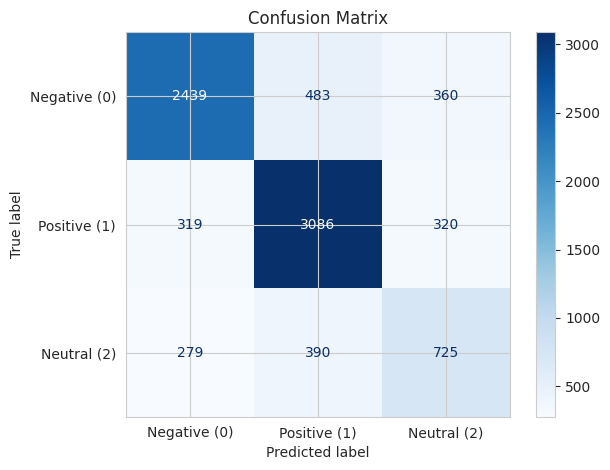
\includegraphics[width=1.0\linewidth]{confusion_matrix.png}
      \captionof{figure}{Confusion Matrix}
    \end{column}
    \begin{column}{0.35\textwidth}
      \centering
      \scriptsize
      \begin{tabular}{@{}lrrrr@{}}
        \toprule
        & \textbf{prec} & \textbf{recall} & \textbf{f1} & \textbf{support} \\
        \midrule
        Neg (0) & 0.80 & 0.74 & 0.77 & 3282 \\
        Pos (1) & 0.78 & 0.83 & 0.80 & 3725 \\
        Neut (2) & 0.52 & 0.52 & 0.52 & 1394 \\
        \midrule
        accuracy & & & 0.74 & 8401 \\
        macro avg & 0.70 & 0.70 & 0.70 & 8401 \\
        weighted avg & 0.74 & 0.74 & 0.74 & 8401 \\
        \bottomrule
      \end{tabular}
      \captionof{table}{Classification Report}
    \end{column}
  \end{columns}
\end{frame}

% Sample Predictions Table (Optional)
\begin{frame}{Sample Predictions on Unseen Data}
  \centering
  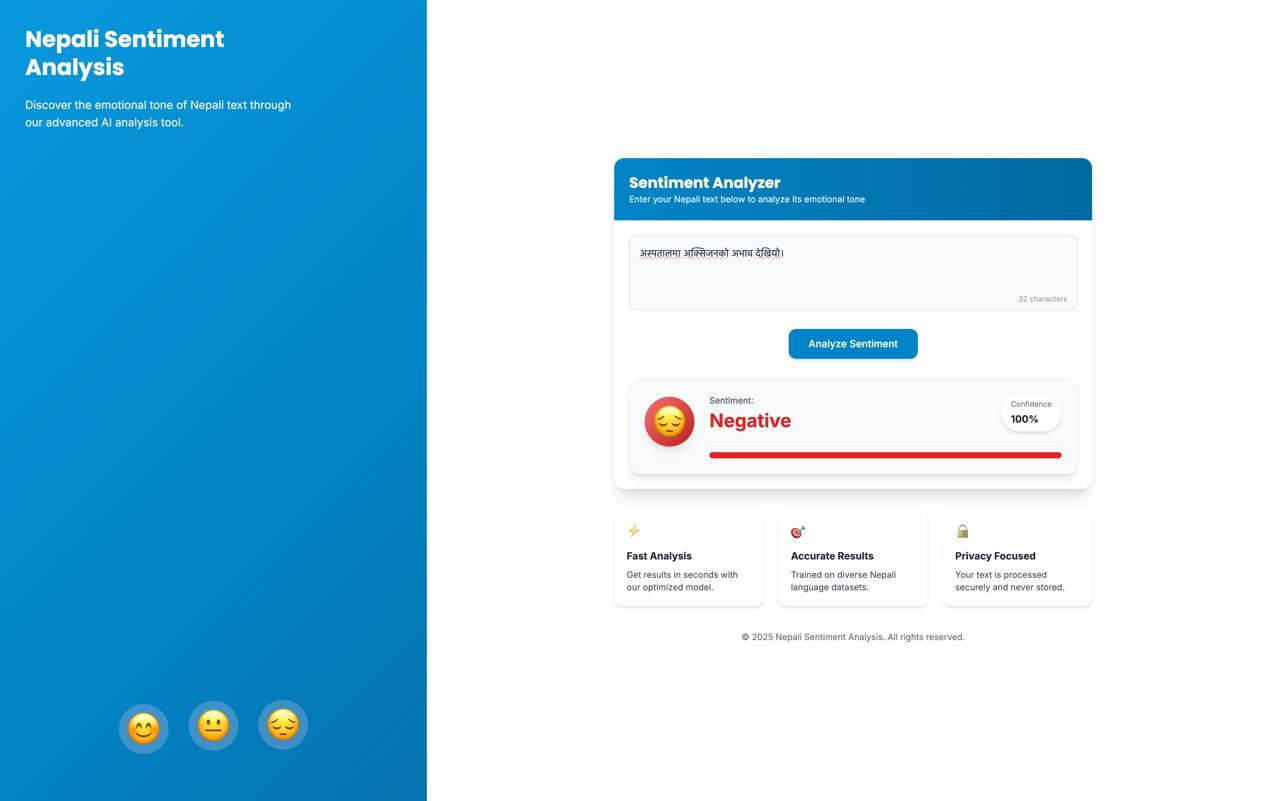
\includegraphics[width=0.75\linewidth]{visual.jpeg}
    \captionof{figure}{Sample Prediction}
\end{frame}

% Conclusion slide
\section{Conclusion}
\begin{frame}{Conclusion and Future Work}
  Key Takeaways:
  \begin{itemize}
    \item Trained a sentiment classifier on Nepali-language text using XLM-Roberta \parencite{conneau-etal-2020-unsupervised,timilsina-etal-2022-nepberta}.
    \item Achieved ~74\% of overall accuracy.
    \item Strong performance on binary sentiment; neutral remains challenging.
  \end{itemize}

  Future Improvements:
  \begin{enumerate}
    \item Larger or augmented datasets.
    \item Additional validation set for tuning.
    \item Model deployment as an API/web service \parencite{fastapi}.
  \end{enumerate}
\end{frame}

% Thank You Slide
\begin{frame}{Thank You!}
  \centering
  Questions or feedback?

  \vspace{2em}

  Project Resources:

  {\footnotesize
  GitHub: {\texttt{\href{https://github.com/saileshbro/ai-proj}{github.com/saileshbro/ai-proj}}}}

  \vspace{2em}

  We appreciate your time and attention!
\end{frame}

\begin{frame}[allowframebreaks]
  \printbibliography
\end{frame}


\end{document}
